\documentclass{article}

% Language setting
% Replace `english' with e.g. `spanish' to change the document language
\usepackage[english]{babel}

% Set page size and margins
% Replace `letterpaper' with `a4paper' for UK/EU standard size
\usepackage[letterpaper,top=2cm,bottom=2cm,left=3cm,right=3cm,marginparwidth=1.75cm]{geometry}

% Useful packages
\usepackage{amsmath}
\usepackage{graphicx}
\usepackage[colorlinks=true, allcolors=blue]{hyperref}

\title{TDT4171 — Artificial Intelligence Methods \\ Assignment 6 - Learning from observations}
\author{Erik Storås Sommer - 535006}
\date{March 2023}

\begin{document}
\maketitle
\setlength{\parindent}{0pt}

\section*{Exercise 1}

\subsection*{Info}

For debugging and learning purposes, I have used graphviz to visualize the decision trees.
May therefor need to run 'pip install graphviz' to get the code to run if it is not already installed.
The implementation takes advantage of the fact that the attributes and class can only take the values 1 and 2.
This made the information gain calculation faster.

\subsection*{Performance}

Running the code and measuring the time it takes iterating 100 times, and then calculating the mean and variance, we get the following results:

\begin{figure}[h]
    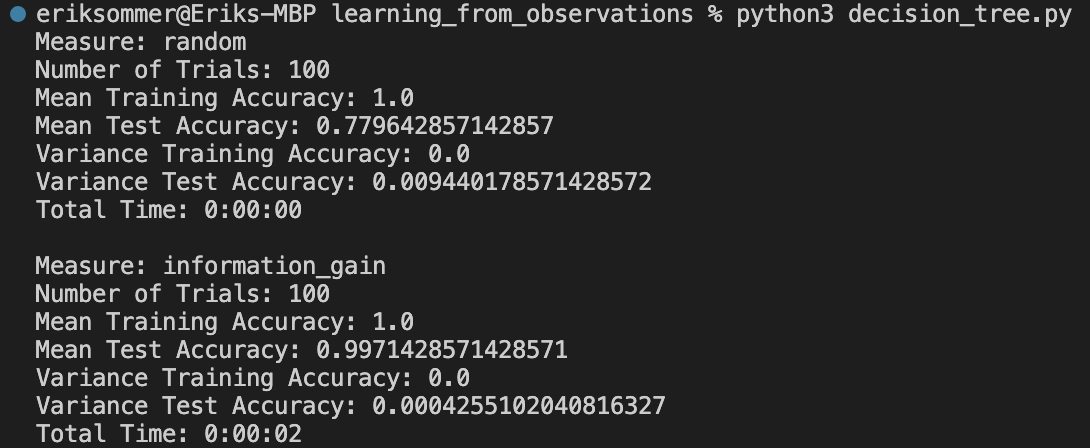
\includegraphics[width=\linewidth]{output.png}
    \caption{Output from running the code}
    \label{fig:image1}
\end{figure}

We see that the time it takes to run the algorithm that allocate a random number as importance to each attribute is under 1 second, while the time it takes to run the algorithm that allocate the expected information gain as importance to each attribute is around 2 seconds.
This is due to the exstra calculations that need to be done to calculate the expected information gain.
On the other hand we see that the accuracy of the decision tree using information gain is much higher than the one using random.
This is because the information gain is a better measure of how much information an attribute gives us about the class.
The variance is also less than for random allocation.

\subsection*{Decision trees}

Below we see that the decision tree using random allocation is much more complex and has a greater depth than the one using information gain.
This makes the decision tree using the information gain more generalizable and less likely to overfit the data.

\begin{figure}[t]
    \centering
    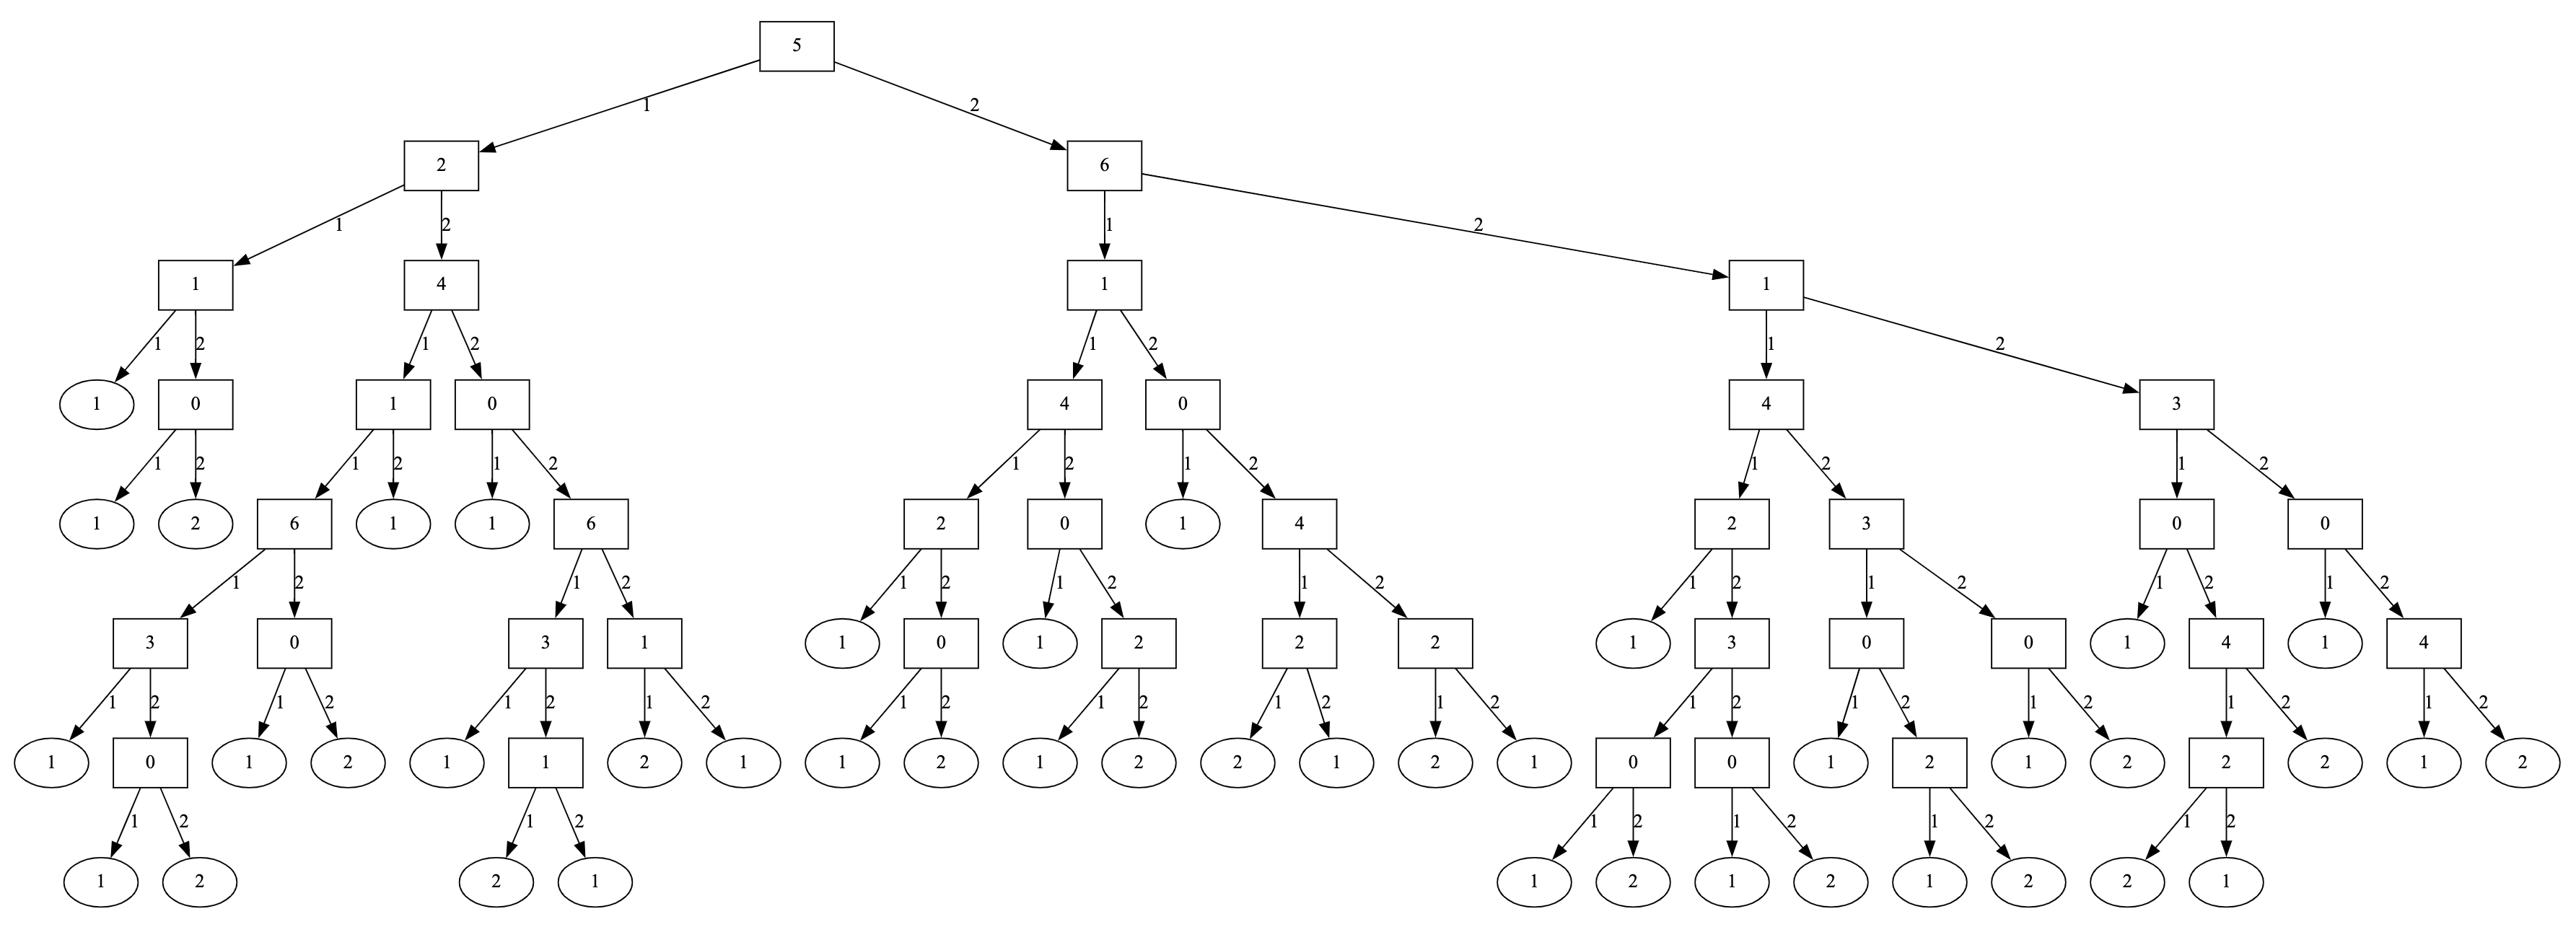
\includegraphics[width=\linewidth]{random.png}
    \caption{Decision tree using random number as importance to each attribute}
    \label{fig:image2}
\end{figure}

\begin{figure}[t]
    \centering
    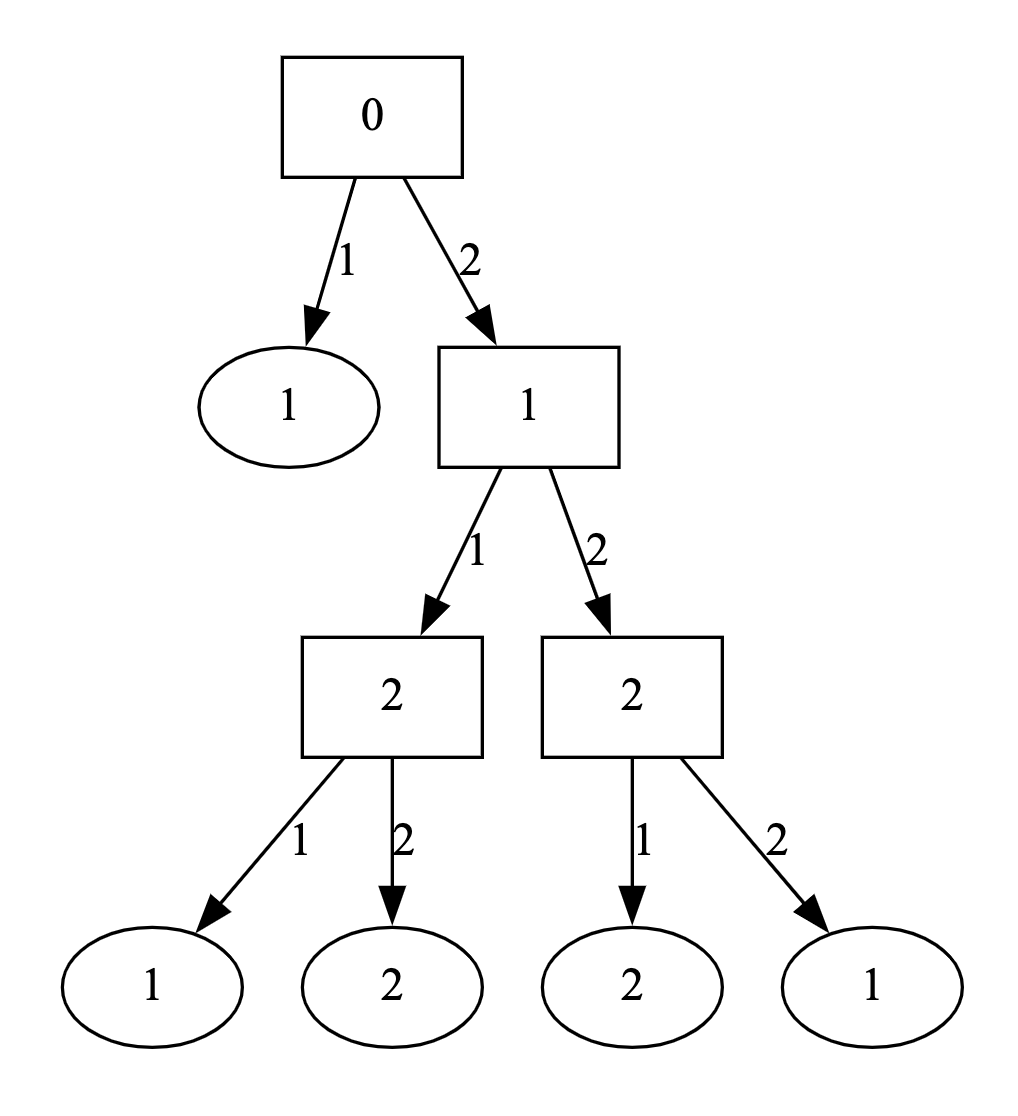
\includegraphics[width=0.5\textwidth]{information_gain.png}
    \caption{Decision tree using the expected information gain as importance to each attribute}
    \label{fig:image3}
\end{figure}

\subsection*{Conclution}

We see that the expected information gain is a better measure of how much information an attribute gives us about the class than a random number, though it is more computationally expensive to calculate.

\end{document}